\chapter{Achievement}

\section{Presentation}

This project consisted firstly to make a detailed study of Android:
\begin{description}
    \item[$\Rightarrow$ Its market;]
    \item[$\Rightarrow$ Its potential;]
    \item[$\Rightarrow$ Its future.]
\end{description}

\noindent Following this study, a document presenting this study was then performed.
Then the second part of the project was to learn application development using the Android Eclipse software and the emulator included in the SDK for Android.
Examples of functional applications have been developed to improve and better understand the subject.
The third part, the most important, was the development of a functional application : in this case, a task manager. This application was developed using version 2.2 of Android (Froyo) and was tested under the latest release, currently, 2.3 (Gingerbeard). The application is internationalized and can therefore choose the language (English or French).

\noindent In the next parts of the report will be presented the different features of the application made during the project.

\section{Home screen}

When launching the application on his Smartphone or on the emulator, the home screen below appears.

\begin{figure}[!ht]
    \centering
    
\includegraphics[height=6cm]{home.png}
    \caption{Home Screen of the application}
\end{figure}

\noindent The top bar displays the application name and the number of tasks it has.
At the top of the homepage, is situated 3 buttons. Between them is displayed the name of the current task. The first button takes you back to the display of all root tasks (tasks that have no daughter). The second takes you back to the parent task and the third adds a new sub-task to the current task.
At the center of the screen, the list of tasks already created and appears contains the main task: name, description, date, number of subtasks. To the right of each task is a blue button that provides access to sub-tasks of that task. To edit a task, just simply press it, a new window will open.
If the user wants to access the various options in the application, he may press the "Menu" of its Smartphone. A menu will then appear at the bottom of the screen (see image above) and will sort, sync, add a tag ...

\noindent When the user changes the screen orientation of his smartphone, it automatically resizes the window with the list of tasks.

\begin{figure}[!ht]
    \centering
    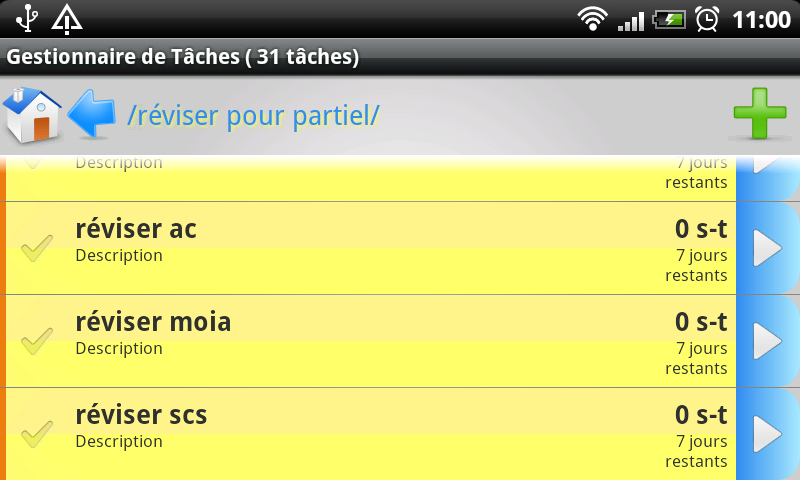
\includegraphics[height=6cm]{orientation.png}
    \caption{Change of orientation}
\end{figure}

\section{Information of a task}

When you click on a task to edit it or when you create a task, a form appears with the different task information (name, description, status, priority, date, tags). This page allows you to modify (or add) the information in a task, when finished, you press the button "back", the task is saved and then you get on the main page with the new list tasks.

\begin{figure}[!ht]
    \centering
    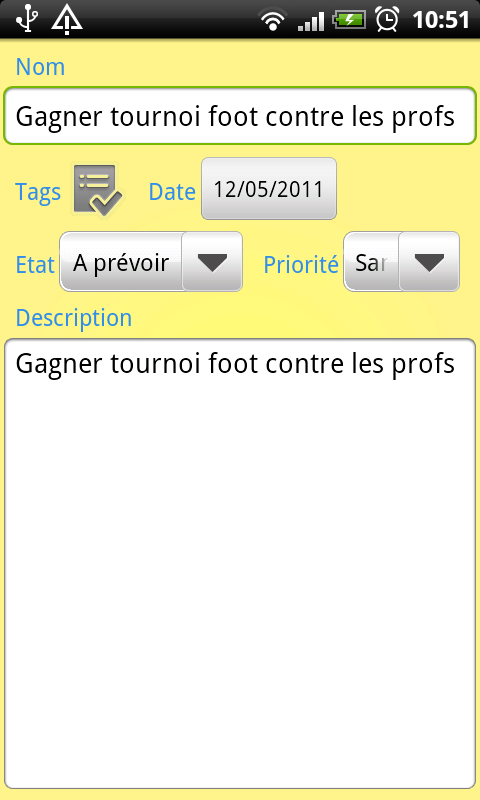
\includegraphics[height=6cm]{details.png}
    \caption{Information of a task}
\end{figure}

\section{Tag management}

A task can have one or more tags. These allow you to group tasks. For this, the user can sort the tasks according to their tag by pressing the "Menu" and selecting "Sort". He can also remove or add tags using the menu.

\begin{figure}[!ht]
    \centering
    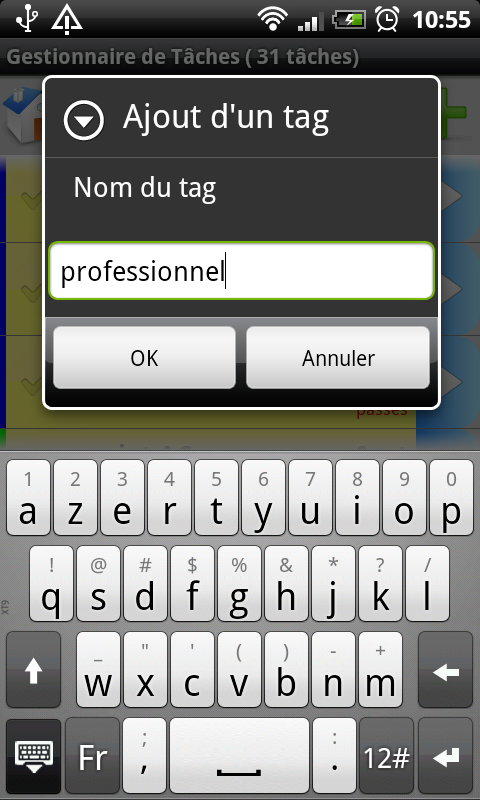
\includegraphics[height=6cm]{tag.png}
    \caption{Add a tag}
\end{figure}

\section{Preferences}

The management of preferences lets users modify settings of the application. To get there, the user can press the menu button and select Settings. It allows the user to choose whether they wish to use a user account (password and login), use a proxy (address and port) or if he wants to display spots canceled.

\begin{figure}[!ht]
    \centering
    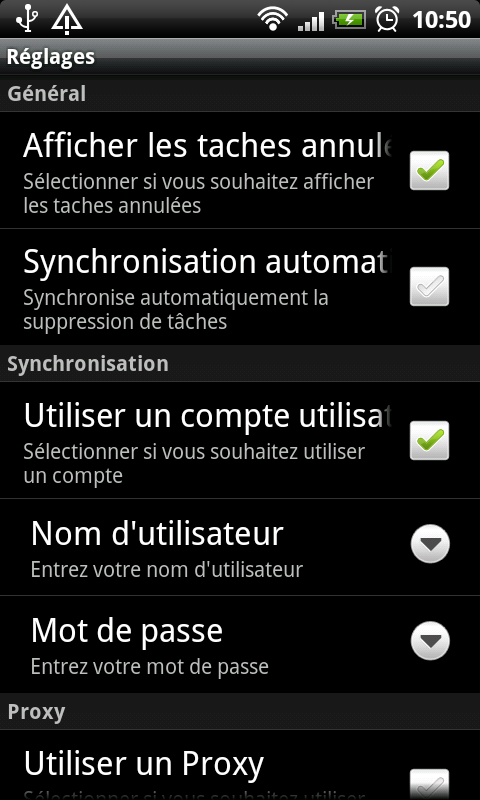
\includegraphics[height=6cm]{prefs.png}
    \caption{Preferences of the application}
\end{figure}

\section{Add an user account}

Management is achieved through synchronization, including user accounts. Indeed, the server can save a list of tasks and tags associated with a user. Therefore, if the application user wants to synchronize its activities on the server, you must first create a user account using the menu "Add User".
To do so, he enters the requested information (name, password, mail, ...), a message will indicate if the account has been created and if he wants to connect automatically. Otherwise, he can always connect later in the application preferences.

\begin{figure}[!ht]
    \centering
    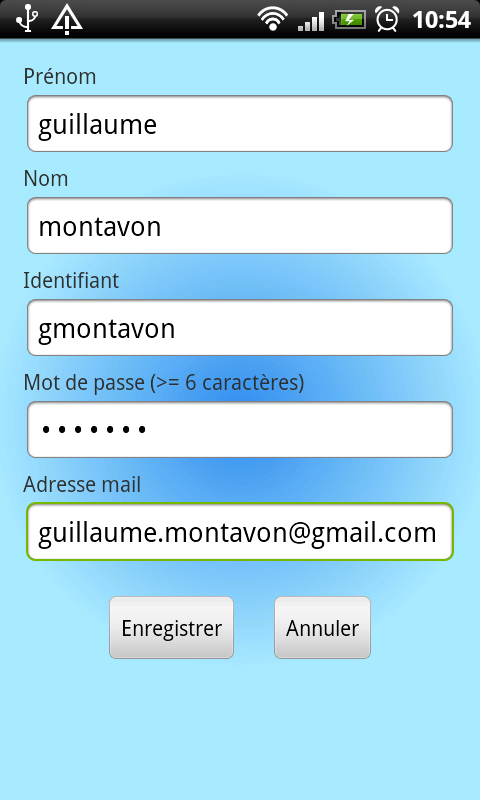
\includegraphics[height=6cm]{add_user.png}
    \caption{Add an user account}
\end{figure}

\section{Synchronization}

There are already many task manager on the Android Market, but the main advantage of this application is that users can synchronize their tasks on a remote server.
3 synchronization modes are available:
\begin{description}
    \item[$\Rightarrow$ Overwrite] the server with the mobile;
    \item[$\Rightarrow$ Crush] the mobile data server;
    \item[$\Rightarrow$ Combining data] from the server with those of the Smartphone.
\end{description}

\begin{figure}[!ht]
    \centering
    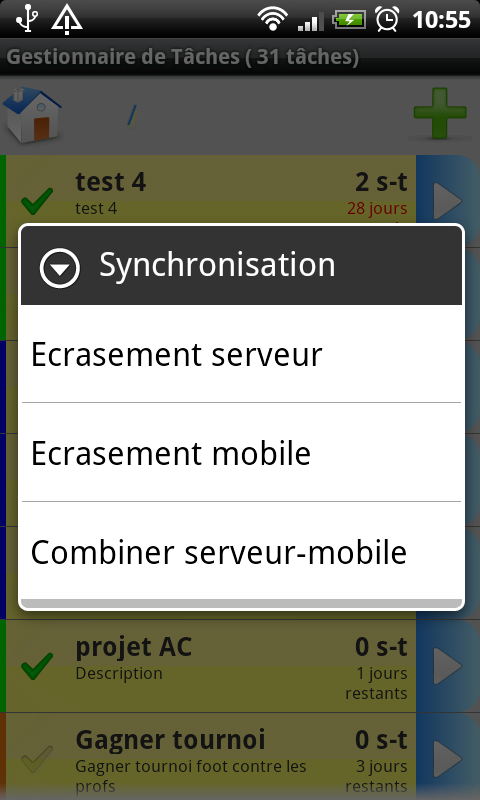
\includegraphics[height=6cm]{synchronise.png}
    \caption{Choice of synchronization mode}
\end{figure}

\noindent To synchronize its tasks on the remote server, the user must first create a user account (see previous section), then enter their username and password in the settings of the application (see chapter on preferences). He can, then, synchronize his tasks by going to the menu, then pressing "Sync" and then finally by selecting the mode of synchronization which he wishes.

\noindent The data sent between the remote server and the Smartphone are encoded in JSON. The remote server has been coded in PHP during the project.

\clearpage
